\chapter{匹配问题(Matching Problem)}

\begin{introduction}
	\item 定义
	\item 算法设计
	\item 算法分析
\end{introduction}

\section{问题引入}\label{sec:stable-matching-def}
现在有n个男性的一个集合$M=\{m_1,\dots,m_n\}$和n个女人性一个集合$W=\{w_1,\dots,w_n\}$。
用$M\times W$来表示$(m,w)$所有可能有序对的一个集合,其中$m\in M,w\in W$。一个匹配(Matching)$S$是一个有序对的集合,
这些有序对来自于$M\times W$,并且每一个来自$M$中的元素和来自$W$中的元素最多在$S$中出现一次。
一个完美匹配(Perfect Matching)$S'$是指每一个来自$M$和$W$中的元素都出现过一次的匹配。
\begin{definition}{匹配(Matching)}{matching}
	对于一个给定的0图$G=(V,E)$,这幅图的一个匹配$M$是图$G$的一个子图(由原来的图的一部分顶点和一部分边构成的图),其中每两条边都不相邻(没有公共顶点)。
	在匹配图中,一个顶点连出的边数至多是一条。如果这个顶点连出一条边,就称这个顶点是已匹配的。$M$中的一条边的两个端点叫做在M中是配对的。
\end{definition}
\begin{definition}{完美匹配(Perfect Matching)}{perfect-matching}
	完美匹配是一个包括了图G中原来的所有顶点的匹配。
\end{definition}
现在我们添加优先级的概念。每一个男性$m\in M$对所有的女性有一个排名。如果在$m$的排名中$w$比$w'$更高,我们说m相对于$w'$更倾向于$w$。
我们把$m$的有序评价叫做他的倾向列表。在$m$的评价中所有人的排名都不相同。类似的,对于每一个$w\in W$也对所有的男性有个排名。

\begin{wrapfigure}[10]{r}{0.25\linewidth}
	\centering
	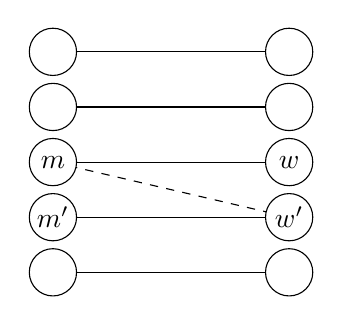
\begin{tikzpicture}
		\draw[dashed] (0,5-0.7*3)  -- (3,5-0.7*4);
		\foreach \x in {5,...,1}
			{
				\draw (0,5-0.7*\x) -- (3,5-0.7*\x);
				\filldraw [fill=white] (0,5-0.7*\x) circle (0.3) node[](m-\x){} (3,5-0.7*\x) circle (0.3) node[](w-\x){};
			}
		\draw
		(m-3) node(){$m$}
		(m-4) node(){$m'$}
		(w-3) node(){$w$}
		(w-4) node(){$w'$};
	\end{tikzpicture}
	\caption{不稳定的情况}
	\label{fig:stable-matching-1}
\end{wrapfigure}
给定一个完美匹配$S$,我们应该担心下面的情况(如\autoref{fig:stable-matching-1})。现在有两个$S$中的匹配$(m,w)$和$(m',w')$,但$m$相对于$w$更倾向于$w'$,
并且$w'$相对于$m'$更倾向于$m$。在这种情况下,没办法阻止$m$和$w'$放弃当前的对象然后组成新的一对。在这种情况下,我们说$(m,w')$对于$S$来说是个不稳定的对。
也就是说,尽管$(m,w')$不存在于$S$中,但$m$和$w'$,相对于他们在$S$中的同伴,更倾向于彼此。

我们的目标是找到一个匹配,这个匹配是完美匹配,并且没有不稳定的对。这个匹配也叫稳定匹配。
\begin{definition}{稳定匹配(Stable Matching)}{stable-matching}
	稳定匹配是一个满足以下条件的匹配:
	\begin{enumerate}[label=(\roman*)]
		\item 是一个完美匹配
		\item 不存在不稳定的的对
	\end{enumerate}
\end{definition}

\section{算法设计}\label{sec:stable-matching-algorithm}
依据上文提到的问题,我们来考虑一下求解方法。
\begin{itemize}[label=$\ast$]
	\item 在最一开始,每个人都是未匹配的。设想一个未匹配的男性$m$选择了在他倾向列表中排名最高的女性$w$,
	      并且提出了请求。所以我们能立刻声明$(m,w)$是我们最后稳定匹配中的一个对吗?不行,在后面有可能$m'$,
	      他在$w$的排名更高,同样向$w$提出了请求。在另一方面,$w$立刻拒绝$m$也是有风险的。她可能不会再收到
	      排名比$m$高的人发出的请求。所以,一个自然地想法是将$(m,w)$对置成约定状态(\sout{约会})。
	\item 假定我们现在处于某个状态,部分是没有匹配的,部分是处于约定状态的。下一步就是一个未匹配的$m$选择了
	      $m$还没有申请过的排名最高的$w$,向$w$提出申请。如果$w$是未匹配的,那么$m$和$w$就成为约定状态。
	      如果$w$是跟$m'$处于约定状态,在这种情况下,$w$根据$m$和$m'$谁的排名更高来选择跟谁成为约定状态,
	      而另一个人就成了未匹配状态。
	\item 最后,这个算法会在没有人处于未匹配状态时停止。这时,所有处于约定状态的就成为最终的结果,
	      得到了一个稳定匹配。
\end{itemize}
\autoref{alg:gale-shapley-algorithm}就是盖尔-沙普利算法(Gale-Shapley algorithm)的具体描述。
\begin{algorithm}
	\caption{盖尔-沙普利算法(Gale-Shapley algorithm)}\label{alg:gale-shapley-algorithm}
	\KwData{男性集合$M$,女性集合$W$}
	\Begin{
		将$m\in M$和$w\in W$置为未匹配状态。\\
		\While{还有$m\in M$处于未匹配状态并且在他的倾向列表中还有未申请过的}{
			选择一个处于未匹配状态的$m$\\
			选择一个$m$还没有提出过申请的排名最高的$w\in W$\\
			\eIf{$w$是未匹配的}{
				$(m,w)$成为约定状态
			}($w$现在跟$m'$处于约定状态){
				\eIf{相比于$m$,$w$更倾向于$m'$}{
					$m$依然是未匹配的状态
				}(相比于$m'$,$w$更倾向于$m$){
					$(m,w)$成为约定状态\\
					$m'$变成未匹配状态
				}
			}
		}
	}
	\KwResult{将所有的约定状态转化成匹配状态后得到一个稳定匹配}
\end{algorithm}

\section{算法分析}\label{sec:stable-matching-analyze}
通过上述算法,我们可以得到如下命题
\begin{theorem}{}{stable-matching-1}
	$w$从第一次被申请后始终处于约定状态,并且$w$的对象会越来越好。
\end{theorem}
从$m$的视角会完全不同。随着时间的流逝,他会在未匹配和约定状态之间转换。
但下面的命题始终成立
\begin{theorem}{}{stable-matching-2}
	在$m$的优先列表中,$m$请求的对象的排名越来越低
\end{theorem}
下面说明算法是会终止的。
\begin{theorem}{}{stable-matching-3}
	G-S算法最终会在$n^2$次循环后终止
\end{theorem}
给出一个显然的证明。
\begin{proof}
	在本算法中,每次迭代都会选择一个未匹配的$m$向他还没有申请过的$w$提出申请。
	我们令$P(t)$来表示在第t次迭代后,$m$向$w$提出过申请的对$(m,w)$的集合。
	对于任何的t,$P(t+1)$相对于$P(t)$一定是严格增长的。
	所有的$M$和$W$组成的对一共有$n^2$个,所以$P(t)$的值在本算法中最多为$n^2$。
	所以上面的算法最多会在$n^2$后停止。
\end{proof}
下面是一些不显然的结论
\begin{theorem}{}{stable-matching-4}
	如果某个时刻$m$是自由的,那么一定有一个$w$他还没有申请过。
\end{theorem}
\begin{proof}
	假定某个时刻$m$是未匹配的,但他已经向所有的女性提出了申请。那么根据定理\ref{thm:stable-matching-1},每一个女性都处于约定的状态。
	既然约定状态是一个匹配,那么就必然有n个男性处于约定的状态。但一共只有n个男性,而$m$是未匹配的,这就产生了矛盾。
\end{proof}
\begin{theorem}{}{stable-matching-5}
	当算法结束时得到的匹配集合$S$一定是一个完美匹配。
\end{theorem}
\begin{proof}
	约定的对最后会形成匹配。我们袈裟算法会在还有一个未匹配的$m$的时候终止。在终止的时候,$m$一定向所有的女性发出过请求,否则算法不会终止。
	但这与定理\ref{thm:stable-matching-4}矛盾,不可能有向所有的女性申请过后还有未匹配状态的男性。
\end{proof}
最后,我们得到算法的结果是一个稳定匹配
\begin{theorem}{}{stable-matching-6}
	集合$S$是运行G-S算法后得到的配对的集合。则$S$是一个稳定匹配。
\end{theorem}
\begin{wrapfigure}[6]{r}{0.25\linewidth}
	\centering
	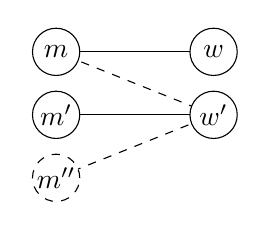
\begin{tikzpicture}
		\draw (0,1.6) node[](m-1){} (2,1.6) node[](w-1){};
		\draw (0,0.8) node[](m-2){} (2,0.8) node[](w-2){};
		\draw (0,0) node[](m-3){};
		\draw (m-1) -- (w-1) (m-2) -- (w-2);
		\draw[dashed] (m-1) -- (w-2) -- (m-3) ;
		\filldraw[fill=white] (m-1) circle (0.3) (m-2) circle (0.3) (w-1) circle (0.3) (w-2) circle (0.3);
		\fill [fill=white] (m-3) circle (0.3);
		\draw [dashed] (m-3) circle (0.3);
		\draw (m-1) node(){$m$} (m-2) node(){$m'$} (w-1) node(){$w$} (w-2) node(){$w'$} (m-3) node(){$m''$};
	\end{tikzpicture}
	\caption{}\label{fig:stable-matching-2}
\end{wrapfigure}
\begin{proof}
	由定理\ref{thm:stable-matching-5},集合$S$是一个完美匹配。所以要证明$S$是一个稳定匹配,我们可以假定$S$中存在不稳定的对,然后推出矛盾。
	假定$S$中有两个匹配对$(m,w)$和$(m',w')$,并且具有下面的特点
	\begin{itemize}[label=$\ast$]
		\item 相比于$w$,$m$更倾向于$w'$
		\item 相比于$m'$,$w'$更倾向于$m$
	\end{itemize}
	在执行算法的过程中,当$m$向$w$提出申请时,$m$是不是已经向$w'$提出过申请?如果没有,那么$w$在$m$的评价中比$w'$更高,这跟我们的假设“相比于$w$,$m$更倾向于$w'$”矛盾。
	如果$m$已经提出过申请,那么他被$w'$选择了更倾向的$m''$时拒绝了。$m'$是$w'$的最终选择,所以$m'$的在$w'$中的排名不会比$m''$低。这与假设“相比于$m'$,$w'$更倾向于$m$”矛盾。
	所以集合$S$中不存在不稳定对,$S$是个稳定匹配。
\end{proof}
下面来说明一下G-S算法得到的解是相同的。书上说有一种简单的方法来证明这一点(\sout{我没看出来})。我们可以证明得到的解具有相同的特征。然后再得到解是相同的。

首先,如果存在一个稳定匹配包含对$(m,w)$,我们可以说$w$是$m$的一个有效同伴。如果$w$是$m$的一个有效同伴,并且在$m$的排名中比$m$的其他的有效同伴都要高,那么可以说$w$是$m$的最佳有效同伴。
我们用$best(m)$来表示$m$的最佳有效同伴。现在假定$S^*$是一个满足$S^*=\{(m,best(m)):m\in M\}$的对集合。我们将要证明下面的定理。
\begin{theorem}{}{stable-matching-7}
	每一次执行G-S算法得到的结果都是集合$S^*$。
\end{theorem}
\begin{wrapfigure}[]{r}{0.25\linewidth}
	\centering
	\begin{tikzpicture}
		%元素关系
		\draw (0,1.6) node[](m-1){} (2,1.6) node[](w-1){};
		\draw (0,0.8) node[](m-2){} (2,0.8) node[](w-2){};
		\draw (0,0) node[](m-3){};
		\draw[dashed] (m-1) -- (w-1) (m-2) -- (w-2);
		\draw (m-2) -- (w-1) ;
		\filldraw[fill=white] (m-1) circle (0.3) (m-2) circle (0.3) (w-1) circle (0.3) (w-2) circle (0.3);
		\fill [fill=white] (m-3) circle (0.3);
		\draw (m-1) node(){$m$} (m-2) node(){$m'$} (w-1) node(){$w$} (w-2) node(){$w'$};
		%图例
		\draw[dashed] (-0.3,0)--(0,0) node[right](){集合$S'$};
		\draw (-0.3,-0.5)--(0,-0.5) node[right](){集合$S$或过程$\varepsilon$};
	\end{tikzpicture}
	\caption{}\label{fig:stable-matching-3}
\end{wrapfigure}
\begin{proof}
	我们假定,某次执行G-S算法得到的匹配$S$,其中存在男性没有匹配到他的最佳有效同伴。我们把这个过程记为$\varepsilon$。既然男性提出申请的次序是沿着倾向列表降序的,
	那也就是说存在男性在$\varepsilon$中被他的有效同伴被拒绝了。%根据定理\ref{thm:stable-matching-2},也就是存在男性$m$被他的最佳有效同伴$ws$拒绝了。
	那么在$\varepsilon$中,记第一个被有效对象拒绝的为$m$,并且被他的有效对象$w$拒绝。
	考虑$m$被$w$拒绝的时刻,要么是因为$w$已经跟排名更高的$m'$成了约定状态,要么是因为排名更高的$m'$向$w$提出了申请。不管怎样,在那个时刻$w$跟$m'$形成或维持约定状态,$m'$在$w$的排名中比$m$要高。

	既然$w$是$m$的一个有效同伴,那么存在一个稳定匹配$S'$包含这个对$(m,w)$。那么,假定这个时候跟$m'$组成对的是$w'$,并且$w‘\neq w$。

	在$\varepsilon$中,$m$是第一个被$w$拒绝的有效对象,那么当$m'$向$w$提出申请的时候还没有被有效对象(比如$w'$)拒绝过,也就是说在$m'$看来$w$的排名比$w'$要高。
	并且$m'$在$w$的排名比$m$要高。那么$(m,w')$在$S'$中倾向成为一对,但$(m,w')\notin S'$,这就是个不稳定因素。

	这跟我们关于$S'$是稳定匹配的声明是矛盾的,因此我们最初的声明是错误的。那么不存在任何过程使得$m$不与最佳有效同伴$best(m)$匹配。
\end{proof}
对于男性,G-S算法得到的是理想的。不幸的是对于女性来说是不一样的。对于一个女性$w$,如果存在一个稳定匹配包含对$(m,w)$,那么我们说$m$是一个有效同伴。如果$m$是$w$的一个有效同伴,
并且对于$w$来说没有有效同伴的排名比$m$低,那我们说$m$是$w$的最差有效同伴。
\begin{theorem}{}{stable-matching-8}
	在稳定匹配$S^*$中,每一个女性都跟她的最差有效同伴匹配。
\end{theorem}
\begin{wrapfigure}[]{r}{0.25\linewidth}
	\centering
	\begin{tikzpicture}
		%元素关系
		\draw (0,1.6) node[](m-1){} (2,1.6) node[](w-1){};
		\draw (0,0.8) node[](m-2){} (2,0.8) node[](w-2){};
		\draw (0,0) node[](m-3){};
		\draw[dashed] (m-1) -- (w-2) (m-2) -- (w-1);
		\draw (m-1) -- (w-1) ;
		\filldraw[fill=white] (m-1) circle (0.3) (m-2) circle (0.3) (w-1) circle (0.3) (w-2) circle (0.3);
		\fill [fill=white] (m-3) circle (0.3);
		\draw (m-1) node(){$m$} (m-2) node(){$m'$} (w-1) node(){$w$} (w-2) node(){$w'$};
		%图例
		\draw[dashed] (-0.3,0)--(0,0) node[right](){集合$S'$};
		\draw (-0.3,-0.5)--(0,-0.5) node[right](){集合$S^*$};
	\end{tikzpicture}
	\caption{}\label{fig:stable-matching-3}
\end{wrapfigure}

\begin{proof}
	假定存在对$(m,w)$在稳定匹配$S^*$中,并且$m$不是$w$的最差有效同伴。那么存在一个稳定匹配$S'$,$w$跟一个比$m$差的人$m'$形成了对。在$S'$中,$m$跟$w'$形成了一对,且$w'\neq w$。
	由定理\ref{thm:stable-matching-7},我们知道$w$是$m$的最佳有效对象,并且$w'$是$m$的有效对象,那么我们可以说相对于$w'$,$m$更倾向于$w$。
	但这会导致$(m,w)$成为$S'$中的不稳定因素,这与$S'$是稳定匹配是矛盾的。因此我们的假设是错误的。即对于在$S^*$中的$(m,w)$,$m$是$w$的最差有效同伴。
\end{proof}
